\documentclass{article}

% if you need to pass options to natbib, use, e.g.:
%     \PassOptionsToPackage{numbers, compress}{natbib}
% before loading neurips_2026

% The authors should use one of these tracks.
% Before accepting by the NeurIPS conference, select one of the options below.
% 0. "default" for submission
% \usepackage{neurips_2026}
% the "default" option is equal to the "main" option, which is used for the Main Track with double-blind reviewing.
% 1. "main" option is used for the Main Track
%  \usepackage[main]{neurips_2026}
% 2. "position" option is used for the Position Paper Track
%  \usepackage[position]{neurips_2026}
% 3. "eandd" option is used for the Evaluations & Datasets Track
 % \usepackage[eandd]{neurips_2026}
 % if you need to opt-in for a single-blind submission in the E&D track:
 %\usepackage[eandd, nonanonymous]{neurips_2026}
% 4. "creativeai" option is used for the Creative AI Track
%  \usepackage[creativeai]{neurips_2026}
% 5. "sglblindworkshop" option is used for the Workshop with single-blind reviewing
 % \usepackage[sglblindworkshop]{neurips_2026}
% 6. "dblblindworkshop" option is used for the Workshop with double-blind reviewing
%  \usepackage[dblblindworkshop]{neurips_2026}

% After being accepted, the authors should add "final" behind the track to compile a camera-ready version.
% 1. Main Track
%  \usepackage[main, final]{neurips_2026}
% 2. Position Paper Track
%  \usepackage[position, final]{neurips_2026}
% 3. Evaluations & Datasets Track
 % \usepackage[eandd, final]{neurips_2026}
% 4. Creative AI Track
%  \usepackage[creativeai, final]{neurips_2026}
% 5. Workshop with single-blind reviewing
%  \usepackage[sglblindworkshop, final]{neurips_2026}
% 6. Workshop with double-blind reviewing
%  \usepackage[dblblindworkshop, final]{neurips_2026}
% Note. For the workshop paper template, both \title{} and \workshoptitle{} are required, with the former indicating the paper title shown in the title and the latter indicating the workshop title displayed in the footnote.
% For workshops (5., 6.), the authors should add the name of the workshop, "\workshoptitle" command is used to set the workshop title.
% \workshoptitle{WORKSHOP TITLE}

% "preprint" option is used for arXiv or other preprint submissions
% \usepackage[preprint]{neurips_2026}

% to avoid loading the natbib package, add option nonatbib:
% \usepackage[nonatbib]{neurips_2026}

% Using the Purdue Digital Twin Lab report style for preprint on arXiv
\usepackage{pdt_report}

\input{commands}
\definecolor{boilermakergold}{HTML}{cfb991}
\definecolor{steel}{HTML}{555960}
\definecolor{coolgray}{HTML}{6f727b}
\definecolor{dust}{HTML}{EBD99F}
\usepackage{cleveref}
\crefname{corollary}{corollary}{corollaries}
\Crefname{corollary}{Corollary}{Corollaries}

% Change the title of your supplementary material here.
\renewcommand{\appendixtocname}{\Large Supplementary Material}
\renewcommand{\appendixpagename}{\large Supplementary Material}

% Note. For the workshop paper template, both \title{} and \workshoptitle{} are required, with the former indicating the paper title shown in the title and the latter indicating the workshop title displayed in the footnote.
\title{On Variance Reduction in Learning Mean Flows}


% The \author macro works with any number of authors. There are two commands
% used to separate the names and addresses of multiple authors: \And and \AND.
%
% Using \And between authors leaves it to LaTeX to determine where to break the
% lines. Using \AND forces a line break at that point. So, if LaTeX puts 3 of 4
% authors names on the first line, and the last on the second line, try using
% \AND instead of \And before the third author name.


\author{%
  Juanwu~Lu \\
  Purdue University \\
  \texttt{juanwu@purdue.edu}
  \And
  Ziran Wang \\
  Purdue University \\
  \texttt{ziran@purdue.edu}
}


\begin{document}

\maketitle

% -----------------------------------------
% Main contents
\begin{abstract}
    \label{sec: abstract}
    Mean Flows enable distillation-free one-step generation by learning two-parameter average-velocity fields from noise to data distributions, but their training is notorious for non-decreasing loss and high gradient variance. We establish a theoretical framework that explains the phenomenon through the lens of \textit{variance reduction with a control variate}. We identify two distinct statistical roles for the conditional velocity $\vv_{\text{cond}}$ in training: as an unbiased regression target and as the Monte Carlo control variate for the tangent in the Jacobi-vector-product (JVP), but with a statistically suboptimal coefficient. The latter inflates per-step gradient variance and produces the non-decreasing loss. We derive the optimal tangent-mixing coefficient $\beta^{\ast}$ in closed form and show that a family of concurrent works correspond to different practical realizations of the same optimum. To validate the framework, we instantiate the $\beta\!=\!1$ corner via an EMA-derived proxy with a flow-matching anchor and run a controlled $\beta$-sweep ($\beta\!\in\!\{0,0.25,0.5,1\}$) at both toy and DiT-B/4 / ImageNet-$256$ scale. The sweep recovers the predicted bias-variance ordering at every matched-step checkpoint, with $3\!\times\!\sim\!5\!\times$ gradient-variance reduction and up to $54\%$ SW$_{1}$ improvement on 2-D benchmarks, and $\approx\!5\!\times$ reduction in gradient noise ratio at DiT scale. The same DiT-scale measurement also exposes a quantitative \emph{FID-vs-MSE landscape mismatch}: the FID-axis bias amplification across $\beta\!=\!0.5/\beta\!=\!1$ ($\sim\!1.4{:}1$) is sublinear in the gradient-MSE bias coefficient ($1{:}4$), so the FID-optimal $\beta$ shifts beyond the gradient-MSE interior minimizer to the unbiased corner $\beta\!=\!0$.
\end{abstract}

% Outline
%
% In this section, we briefly introduce the background of flow-basec/diffusion generative models and recent advances in one-step generation models.
% My plan for this section consists of four paragraphs:
%
% 1. Kick start the introduction with a paragraph discussing about flow-matching and diffusion models. It ends with the limitation of numerical integration.
% 2. Following tha paragraph, describe the recent advances in one-step generation models, including early works on distillation-based one-step generation followed by the introduction of Mean Flows. The paragraph should end by highlighting the limitations: non-decreasing and high-variance loss.
% 3. Following up on our discussion about the limitations, we introduce the primary theoretical contribution of this work: curvature-variance principle, and highlight how we position our contribution amongst concurrent works.
% 4. Finally, we introduce VaMF, a concrete yet simple method to address the analyzed issue and improve the overall performance and training efficiency of the original Mean Flows.

\section{Introduction}
\label{sec: introduction}

%%%%%%%%%%%%%%%%%%%%%%%%%%%%%%%%%%%%%%%%%
% introduction of flow-based/diffusion
Deep generative models that leverage deep neural networks to learn and generate samples from unknown data distributions have achieved profound success. One of the predominant paradigms adopts flow-based generative models~\cite{chen2018neural,rezende2015variational,dinh2017density,grathwohl2019ffjord,lipman2023flowmatchinggenerativemodeling,tong2024improvinggeneralizingflowbasedgenerative,albergo2023buildingnormalizingflowsstochastic} that learn continuous-time transformations between a simple prior and a target data distribution. The existing conditional flow matching~\cite{lipman2023flowmatchinggenerativemodeling,tong2024improvinggeneralizingflowbasedgenerative} and stochastic interpolant~\cite{albergo2023buildingnormalizingflowsstochastic,albergo2025stochasticinterpolants} enable simulation-free training by regressing a velocity field, achieving sample quality competitive with diffusion models~\cite{sohldickstein2015deep,song2019generative,ho2020denoising,nichol2021improved,song2021scorebased,dhariwal2021diffusion,karras2022elucidating} and variational autoencoders~\cite{kingma2014auto}. However, flow-based models share the same limitation as diffusion models as they require iterative integration at inference time, which can suffer from extensive computational costs and numerical instability.

%%%%%%%%%%%%%%%%%%%%%%%%%%%%%%%%%%%%%%%%%
% few-/one-step generation models
The issue motivates consecutive studies on reducing the number of function evaluations to one or few steps~\cite{song2021denoising}. Existing approaches include progressive distillation~\cite{salimans2022progressivedistillationfastsampling}, distribution matching~\cite{yin2024distributionmatchingdistillation,yin2024improveddistributionmatchingdistillation}, consistency models~\cite{song2023consistencymodels,lu2025simplifyingstabilizingscalingcontinuoustime}, and flow map matching~\cite{boffi2025flowmapmatchingstochastic}, but most require a pre-trained teacher model. Recently, Mean Flows~\cite{geng2025meanflowsonestepgenerative} offers an appealing \textit{distillation-free} alternative by learning a two-parameter average velocity field $\vu(\vx,r,t)$ through a total-derivative identity between the average and marginal velocity field. In principle, this identity provides exact self-supervision. The compound prediction $\vu+(t-r)\frac{\mathrm{d}}{\mathrm{d}t}\vu$ should match the instantaneous velocity at convergence, requiring no external teacher. Nevertheless, empirical training of Mean Flows is plagued by non-decreasing loss and prohibitively high gradient variance~\cite{zhang2025alphaflowunderstandingimprovingmeanflow,geng2025improvedmeanflowschallenges}.

%%%%%%%%%%%%%%%%%%%%%%%%%%%%%%%%%%%%%%%%%
% our contributions
In this work, we conduct a theoretical analysis that attributes the issue to replacing the marginal velocity fields by conditional fields in the total derivatives and the regression target, and establish the \textbf{curvature-variance principle}. Specifically, we prove that: \textbf{(i)} the per-step gradient variance is amplified by a Jacobi factor $\Tr(\mJ\Sigma_{\vv'}\mJ^{\!\top})$ where $\mJ=(t-r)\partial_{\vz}\vu_{\vtheta}-\mI_{d}$, and the stop-gradient operator creates a semi-gradient gap that blinds the optimizer to this amplification; \textbf{(ii)} there exists a connection between the Jacobi and the curvature gap $\Delta:=\vu-\vv$, which satisfies $\Delta\approx-\frac{(t-r)}{2}\frac{\mathrm{D}\vv}{\mathrm{D}t}$, so it is the local flow acceleration that causes the average and instantaneous velocities to diverge; and \textbf{(iii)} the acceleration-to-noise ratio $\text{ANR}=(t-r)\|\frac{\mathrm{D}\vv}{\mathrm{D}t}\|/\sqrt{\Tr(\Sigma_{\vv'})}$ governs the optimal sampling distribution over intervals, connecting scheduling heuristics in prior work to a principled criterion.

Building on this analysis, we propose \textbf{Variance-Aware MeanFlow (VaMF)}, a backbone-preserving training framework that addresses each diagnostic in turn. First, an \textit{EMA velocity anchor} replaces the stochastic JVP tangent with a deterministic estimate, provably eliminating the Jacobi-amplified gradient noise. Then, a \textit{flow-matching anchor} supervises the boundary condition at $r\!\to\!t$, removing the transient bias that an inexact tangent would otherwise introduce. Finally, a closed-form \textit{trace weight} $w\!\propto\!1/(1+\sigma_{t}^{2}\Tr(\mJ\mJ^{\!\top})/d)$ downweights each sample by the local Jacobian-deviation norm. VaMF preserves the original Mean Flow MSE objective and adds only one Jacobian-vector product per step. Our contributions are as follows:
\begin{description}
    \item[\namedlabel{cb: thm}{C1}] We establish the curvature-variance principle, which attributes the non-decreasing, high-variance loss of Mean Flows to a single mechanism---the Jacobi-amplified per-step gradient variance and its connection to the local flow acceleration---and provide the first formal quantification of the semi-gradient gap induced by the stop-gradient operator.
    \item[\namedlabel{cb: vamf}{C2}] We derive VaMF, a backbone-preserving training framework that combines an EMA velocity anchor, a flow-matching anchor, and a Hutchinson-estimated trace weight to eliminate variance amplification and the associated tangent bias.
    \item[\namedlabel{cb: exp}{C3}] Empirically, VaMF improves Sliced Wasserstein-$1$ ($\text{SW}_{1}$) over vanilla MeanFlow by $-23\%$, $-13\%$, $-23\%$, and $-54\%$ on the four 2D datasets, scales favorably from $d{=}2$ up to $d{=}64$ on the dense-Gaussian-mixture sweep, and transfers to large training of latent-space image generation models on the ImageNet datasets.
\end{description}

%%%%%%%%%%%%%%%%%%%%%%%%%%%%%%%%%%%%%%%%%
% Preliminary
%
% In this section, I will briefly discuss conditional flow-matching and Mean Flows for one-step generation
%
\section{Preliminaries}
\label{sec: preliminary}

\noindent\textbf{Flow-Matching.} Let $\vx$ denote a data sample in $\gX\subset\mathbb{R}^{d}$ . Flow-matching generative models~\cite{lipman2023flowmatchinggenerativemodeling,tong2024improvinggeneralizingflowbasedgenerative} learn a time-dependent diffeomorphism $\psi(\vx,t):\mathbb{R}^{d}\!\times\![0,1]\to\mathbb{R}^{d}$ from a simple distribution $\rvx_{1}\!\sim\!{p}(\rvx,1)$ to the target $\rvx_{0}\!\sim\!{p}(\rvx,0)\!=\!\pdata$ by parameterizing a velocity field $\vv(\vx,t)\!\triangleq\!\frac{\mathrm{d}}{\mathrm{d}t}\psi(\vx,t)$. Since the exact \textit{marginal velocity field} $\vv(\vx,t)$ is generally inaccessible, conditional flow-matching~\cite{lipman2023flowmatchinggenerativemodeling} instead learns a conditional field $\vv_{\text{cond}}\!=\!\vx_{1}-\vx_{0}$ with $\vx_{t}\!=\!(1-t)\vx_{0}+t\vx_{1}$. The following lemma justifies the substitution. See~\Cref{appx: first} for its proof.
\begin{lemma}
    Given vector fields $\vv_{\text{cond}}$ generating conditional probability paths $p(\vx,t\mid\vx_{0})$, for any $\rvx_{0}\!\sim\!p(\rvx_{0})$, the expected conditional velocity field is equal to the marginal velocity field
    \begin{equation}
        \vv(\vx,t)=\E_{\vx_{0}\sim{p(\vx_{0}\mid\vx_{t}=\vx)}}\!\left[\vv(\vx,t\mid\vx_{0})\right].
        \label{eq: margv-condv-relation}
    \end{equation}
\end{lemma}

%%%%%%%%%%%%%%%%%%%%%%%%%%%%%%%%%%%%%%%%%
% MeanFlow
%%%%%%%%%%%%%%%%%%%%%%%%%%%%%%%%%%%%%%%%%
\noindent\textbf{One-step Mean Flows.} Iterative integration of $\vv(\vx,t)$ at inference is expensive and can be numerically unstable. To bypass it, Mean Flows~\cite{geng2025meanflowsonestepgenerative} learn a two-parameter average velocity field $\vu(\rvx,r,t)$ through regressing an identity along the flow trajectory $\vx_{\tau}\!=\!\psi(\vx_{r},\tau)$ with terminal at $\vx_{t}\!=\!\vx$:
\begin{equation}
    (t-r)\,\vu(\vx,r,t)=\int_{r}^{t}\vv(\vx_{\tau},\tau)\,\mathrm{d}\tau.
    \label{eq: meanflow-identity}
\end{equation}
Differentiating with respect to the terminal time $t$ along the same trajectory yields
\begin{equation}
    \vu(\vx,r,t)+(t-r)\tfrac{\mathrm{d}}{\mathrm{d}t}\vu(\vx,r,t)=\vv(\vx,t),\qquad
    \tfrac{\mathrm{d}}{\mathrm{d}t}\vu=\partial_{\vx}\vu\!\cdot\!\vv(\vx,t)+\partial_{t}\vu,
    \label{eq: td-meanflow-identity}
\end{equation}
where the total derivative $\frac{\mathrm{d}}{\mathrm{d}t}\vu$ is essentially a JVP, denoted by $\texttt{JVP}(\vu,(\vx,r,t),(\vv(\vx,t),0,1))$. The original MeanFlow paper~\cite{geng2025meanflowsonestepgenerative} replaces \emph{both} occurrences of the marginal field with the conditional field $\vv_{\text{cond}}\!=\!\vx_{1}\!-\!\vx_{0}$, giving the MeanFlow loss
\begin{equation}
    \mathcal{L}_{\text{MF}}(\vtheta)=
    \E_{r,t,\vx_{0},\vx_{1}}\!\left[\left\|\vu_{\vtheta}+(t-r)\,\texttt{sg}\!\left[\texttt{JVP}(\vu_{\vtheta},(\vx_{t},r,t),(\vv_{\text{cond}},0,1))\right]-\vv_{\text{cond}}\right\|_{2}^{2}\right],
    \label{eq: mf-loss}
\end{equation}
with $r,t\!\sim\!\gU(0,1)$, $r\!\leq\!t$, $\vx_{0}\!\sim\!\pdata$, $\vx_{1}\!\sim\!\gN(0,\mI_{d})$, $\vx_{t}\!=\!(1-t)\vx_{0}+t\vx_{1}$, and the stop-gradient $\texttt{sg}[\cdot]$ avoiding double backpropagation through the JVP.

%%%%%%%%%%%%%%%%%%%%%%%%%%%%%%%%%%%%%%%%%%%%%%%%%%%%%%%%%%%%%%%%%%%%%%%%%%%%%%%%
% Variance Reduction in Learning Mean Flows
%%%%%%%%%%%%%%%%%%%%%%%%%%%%%%%%%%%%%%%%%%%%%%%%%%%%%%%%%%%%%%%%%%%%%%%%%%%%%%%%
\section{Variance Reduction in Learning Mean Flows}
\label{sec: method}

The MeanFlow loss in~\eqref{eq: mf-loss} is empirically known to be \textit{non-decreasing} and to suffer from \textit{high-variance gradients}~\cite{zhang2025alphaflowunderstandingimprovingmeanflow,geng2025improvedmeanflowschallenges}. We investigate the statistical mechanism behind this pathology. Importantly, our analysis isolates the role of the conditional velocity field $\vv_{\text{cond}}$ when it appears as the JVP tangent, and identifies that it acts as a Monte Carlo control variate for the inaccessible marginal velocity, with a coefficient that the original MeanFlow fixes to a suboptimal value. We derive the optimal coefficient and establish a connection to practical fixes in concurrent works.

%%%%%%%%%%%%%%%%%%%%%%%%%%%%%%%%%%%%%%%%%
\subsection{Two roles of the conditional velocity field}
\label{subsec: two-roles}

With Reynolds decomposition, we express the conditional velocity by $\vv_{\text{cond}}\!=\!\vv(\vx,t)+\vv^{\prime}$ with $\E_{\vx_{0}\mid\vx_{t}}[\vv^{\prime}]\!=\!\bm{0}$ according to~\eqref{eq: margv-condv-relation} and $\Sigma_{\vv^{\prime}}\!\triangleq\!\Cov_{\vx_{0}\mid\vx_{t}}[\vv^{\prime}]$. The MeanFlow loss in~\eqref{eq: mf-loss} uses $\vv_{\text{cond}}$ both as the \textit{regression target} and as the \textit{tangent} inside the total derivative. Carrying the decomposition through per-sample loss $\ell_{\text{MF}}(\vtheta)$ yields:
\begin{equation}
    \E_{\vx_{0}\mid\vx_{t}}\!\bigl[\ell_{\text{MF}}(\vtheta)\bigr]
    =\bigl\|\vr_{\vtheta}^{\texttt{sg}}\bigr\|^{2}_{2}
    +\texttt{sg}\!\bigl[\Tr(\mJ\Sigma_{\vv^{\prime}}\mJ^{\!\top})\bigr],
    \label{eq: per-sample-expand}
\end{equation}
where $\mJ\!\triangleq\!(t{-}r)\partial_{\vx_{t}}\vu_{\vtheta}\!-\!\mI_{d}\!\in\!\mathbb{R}^{d\times d}$ is a \textit{Jacobi factor} determined by the Jacobian matrix $\partial_{\vx_{t}}\vu_{\vtheta}$ and $\vr_{\vtheta}^{\texttt{sg}}\!\triangleq\!\vu_{\vtheta}\!+\!(t{-}r)\,\texttt{sg}[\partial_{\vx_{t}}\vu_{\vtheta}\!\cdot\!\vv\!+\!\partial_{t}\vu_{\vtheta}]\!-\!\vv$ is the deterministic mean-field residual. Since the residual $\vr_{\vtheta}^{\texttt{sg}}$ is the exact loss we aim to minimize given by~\eqref{eq: td-meanflow-identity}, the trace term leads to the non-decreasing loss and eliminates $\textit{iff}$ the Jacobi satisfies $\partial_{\vx_{t}}\vu_{\vtheta}=\frac{1}{t-r}\mI_{d}$ (equivalently, $\mJ\!=\!\bm{0}$). We identify two roles of the conditional velocity field in this decomposition:

\noindent\textbf{Unbiased Target.} As the regression target, $\vv_{\text{cond}}$ injects $\vv^{\prime}$ \textit{linearly} into the residual, contributing the \emph{irreducible} per-sample noise floor $\Tr(\Sigma_{\vv^{\prime}})$. However, since this noise is independent of $\vtheta$ and $\vv^{\prime}$ is zero-mean, $\vv_{\text{cond}}$ can serve as an unbiased target for learning Mean Flows.

\noindent\textbf{Variance Amplifier.} As the JVP tangent, the same $\vv_{\text{cond}}$ injects $\vv^{\prime}$ \textit{multiplicatively} through the Jacobi factor $\mJ$, contributing the \emph{amplified} term $\Tr(\mJ\Sigma_{\vv^{\prime}}\mJ^{\!\top})$. It scales unboundedly with the spectral magnitude of $\mJ$. This amplification is the dominant driver of variance at the gradient level:

\begin{theorem}[Jacobian Variance Amplification]
    Let $\vg\!\triangleq\!\nabla_{\vtheta}\vu_{\vtheta}(\vx_{t},r,t)\!\in\!\mathbb{R}^{d\times p}$ be the parameter Jacobian of the average velocity. The trace of the conditional gradient covariance (\textit{i.e., the total variance}) of $\ell_{\text{MF}}(\vtheta)$ in~\eqref{eq: mf-loss} satisfies
    \begin{equation*}
        \boxed{
            \Tr\!\left(\Cov\!\left[\nabla_{\vtheta}\ell_{\text{MF}}\mid\vx_{t}\right]\right)
            \;\propto\;
            \Tr\!\left(\vg^{\!\top}\,\mJ\,\Sigma_{\vv^{\prime}}\,\mJ^{\!\top}\,\vg\right).
        }
    \end{equation*}
    \label[theorem]{thm: jacobi-variance}
\end{theorem}

See the proof in~\Cref{appx: theorem-proof}. The theorem identifies that the total gradient variance grows with $\|\mJ\|^{2}$ for fixed $\vg$ and $\Sigma_{\vv^{\prime}}$, saturates only at the irreducible noise floor when $\mJ\!\to\!\bm{0}$, and is \emph{uncontrolled} by any term in the loss due to the use of the stop-gradient in the original MeanFlow. Meanwhile, without the stop-gradient operator, the optimizer could in principle reduce variance by driving $\mJ\!\to\!\bm{0}$. This establishes a \textit{semi-gradient gap}, formally,

\begin{theorem}[Semi-Gradient Gap]
    The gradient of the MeanFlow loss $\gL_{\text{MF}}$ with and without the stop-gradient operator differ by
    \begin{equation}
        \boxed{
            \underbrace{2(t{-}r)\,\E\!\left[\bigl(\nabla_{\vtheta}\!\left(\partial_{\vx_{t}}\vu_{\vtheta}\!\cdot\!\vv+\partial_{t}\vu_{\vtheta}\right)\bigr)^{\!\top}\vr_{\vtheta}\right]}_{\text{mean-field gradient difference}}
            +\underbrace{\E\!\left[\nabla_{\vtheta}\Tr\!\left(\mJ\Sigma_{\vv^{\prime}}\mJ^{\!\top}\right)\right]}_{\text{variance-driven gradient difference}}.
        }
    \end{equation}
    \label[theorem]{thm: semi-gradient-gap}
\end{theorem}

In the original MeanFlow, the stop-gradient operator prevents $\mJ$ from being passed to the optimizer, leading to an empirical non-decreasing loss. Meanwhile, the mean-field difference vanishes at convergence ($\vr_{\vtheta}\!\to\!\bm{0}$) and the variance-driven term $\Tr(\mJ\Sigma_{\vv^{\prime}}\mJ^{\!\top})$ dominates. To better illustrate the idea, \Cref{fig: cm-gap} visualizes the spatial distribution of $\sqrt{\E_{\vx_{0}\mid{\vx_{t}}}\left\|\vv^{\prime}\right\|^{2}}$ on a three-mode, two-dimensional Gaussian mixture. It showcases that the total variance magnitude is non-zero, concentrates in mode-mixing regions where conditional paths overlap, and grows toward the latent endpoint ($t\!\to\!1$).

\begin{figure}[t]
    \centering
    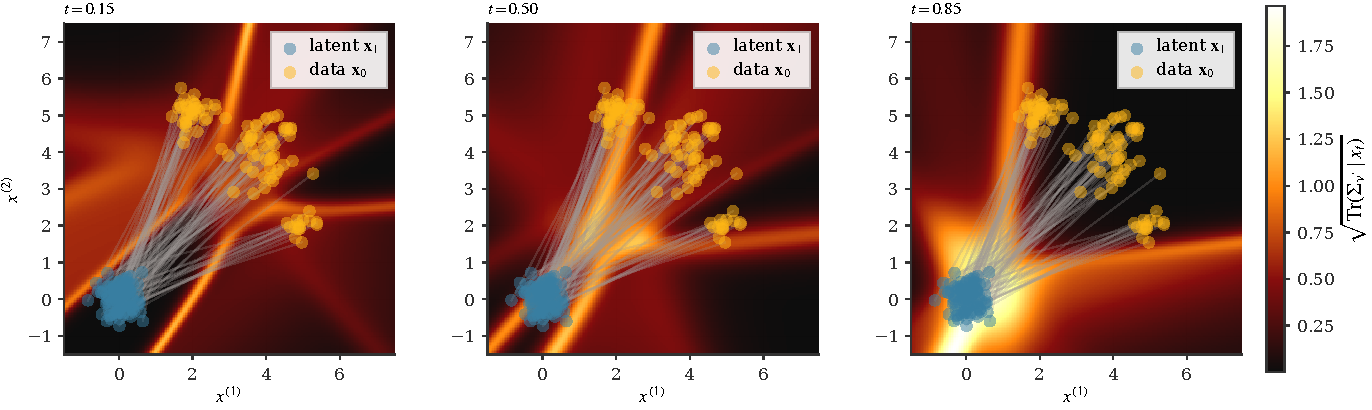
\includegraphics[width=\textwidth]{assets/figures/illustration.pdf}
    \caption{Spatial distribution of $\sqrt{\Tr(\Sigma_{\vv^{\prime}}\!\mid\!\vx_{t})}\!=\!\sqrt{\E_{\vx_{0}\mid\vx_{t}}\|\vv^{\prime}\|^{2}}$ at three timesteps on a two-dimensional Gaussian mixture. Conditional variances concentrate in mode-mixing regions.}
    \label{fig: cm-gap}
    \vspace{-1em}
\end{figure}

%%%%%%%%%%%%%%%%%%%%%%%%%%%%%%%%%%%%%%%%%
\subsection{Rethinking tangent as a control variate}
\label{subsec: control-variate}

The amplification in~\Cref{thm: jacobi-variance} arises due to using $\vv_{\text{cond}}\!=\!\vv\!+\!\vv^{\prime}$ as the JVP tangent injects the zero-mean fluctuation $\vv^{\prime}$. Hence, $\vv_{\text{cond}}$ is analogous to the canonical structure of a Monte Carlo \textit{control variate}~\cite{glasserman2003montecarlo}, where $\vv_{\text{cond}}$ is a stochastic estimator of the inaccessible $\vv$ with known mean, and the coefficient on the noise term $\vv^{\prime}$ determines the bias-variance trade-off. To make this explicit, we introduce a tangent-mixing coefficient $\beta\!\in\![0,1]$:
\begin{equation}
    \tilde{\vv}_{\text{tang}}(\beta)\;\triangleq\;(1-\beta)\,\vv_{\text{cond}} + \beta\,\hat{\vv}\;=\;\vv + (1-\beta)\,\vv^{\prime} + \beta\,\vb,
    \label{eq: tangent-mix}
\end{equation}
where $\hat{\vv}$ can be any deterministic proxy for the marginal velocity (\textit{e.g., a velocity network}) with bias $\vb\!\triangleq\!\hat{\vv}-\vv$ that is deterministic given $\vx_{t}$. Herein, $\beta\!=\!0$ recovers vanilla MeanFlow and $\beta\!=\!1$ replaces the tangent entirely with the deterministic proxy.

\noindent\textbf{Bias-variance trade-off.} Substituting $\tilde{\vv}_{\text{tang}}(\beta)$ for $\vv_{\text{cond}}$ in the JVP tangent and propagating through the loss, the per-sample gradient writes
\begin{equation}
    \vg^{(\beta)} \;=\; 2\,\vg^{\!\top}\!\Bigl[\vr_{\vtheta} \;+\; \bigl((1{-}\beta)\,\mJ - \beta\,\mI\bigr)\,\vv^{\prime} \;+\; \beta\,(\mJ{+}\mI)\,\vb\Bigr],
    \label{eq: g-beta}
\end{equation}
where the noise term scales the conditional fluctuation $\vv^{\prime}$ by the matrix $((1{-}\beta)\,\mJ - \beta\,\mI)$, and the bias term scales the proxy error $\vb$ by $\beta\,(\mJ{+}\mI)$. In this case, we can balance the bias-variance trade-off through solving for the optimal coefficient $\beta^{\ast}$ that minimizes the least-squares between the expected per-sample gradient in~\eqref{eq: g-beta} and the target gradients, given by
\begin{equation}
    M(\beta)\;\triangleq\;\E_{\vv^{\prime}\mid{\vx_{t}}}\left[\left\|\vg^{(\beta)}-\nabla_{\vtheta}\|\vr_{\vtheta}\|_{2}^{2}\right\|_{2}^{2}\right]\;=\;\E_{\vv^{\prime}\mid{\vx_{t}}}\left[\left\|\vg^{(\beta)}-2\vg^{\top}\vr_{\vtheta}\right\|_{2}^{2}\right].
    \label{eq: beta-target}
\end{equation}
We derive the following theorem.

\begin{theorem}[Optimal control-variate coefficient]
    Under the scalar-isotropic approximation $\Sigma_{\vv^{\prime}}\!\approx\!\sigma^{2}\mI_{d}$, $\mJ\!\approx\!\kappa\mI_{d}$, and the parameter-isotropy approximation $\vg\vg^{\!\top}\!\propto\!\mI_{d}$ (which reduces $M$ to a per-component MSE; cf.~\Cref{appx: theorem-proof}),
    \begin{equation*}
        M(\beta) \;\propto\; \beta^{2}(\kappa{+}1)^{2}\|\vb\|^{2} + \sigma^{2}d\bigl((1{-}\beta)\kappa - \beta\bigr)^{2}.
    \end{equation*}
    For $\kappa\!>\!0$, $M(\beta)$ admits a unique minimizer
    \begin{equation}
        \boxed{
            \beta^{\ast} \;=\; \underbrace{\frac{\kappa}{\kappa+1}}_{\text{noise-cancellation}}\;\cdot\;\underbrace{\frac{\sigma^{2}d}{\sigma^{2}d + \|\vb\|^{2}}}_{\text{shrinkage}},
        }
        \label{eq: beta-minimizer}
    \end{equation}
    with optimum value $M(\beta^{\ast})\!\propto\!\sigma^{2}d\,\kappa^{2}\,\|\vb\|^{2}/(\sigma^{2}d+\|\vb\|^{2})$.
    % For all $\kappa,\|\vb\|^{2}\!>\!0$, $M(\beta^{\ast})$ strictly dominates both corner MSEs $M(0)\!\propto\!\sigma^{2}\kappa^{2}d$ (vanilla MeanFlow) and $M(1)\!\propto\!(\kappa{+}1)^{2}\|\vb\|^{2}+\sigma^{2}d$ (deterministic-tangent estimator with bias). The boundary case $\kappa\!=\!-1$ (which corresponds to $\partial_{\vx_{t}}\vu_{\vtheta}\!=\!\bm{0}$ at initialization) leaves $M(\beta)$ constant and is excluded.
    \label[theorem]{thm: control-variate-optimum}
\end{theorem}

See the proof in~\Cref{appx: theorem-proof}. The two components of $\beta^{\ast}$ play distinct roles: $\kappa/(\kappa{+}1)$ is the coefficient that \emph{cancels the Jacobian-amplified noise} through destructive interference between the $\mJ\vv^{\prime}$ and $\mI\vv^{\prime}$ contributions in~\eqref{eq: g-beta}, while $\sigma^{2}d/(\sigma^{2}d{+}\|\vb\|^{2})$ is the standard James-Stein shrinkage~\cite{james1961estimation} that pulls $\beta^{\ast}$ toward the unbiased corner when the proxy bias $\|\vb\|$ is large. Therefore, as the proxy bias shrinks ($\|\vb\|^{2}\!\to\!0$), $\beta^{\ast}\!\to\!\kappa/(\kappa{+}1)$, and as the Jacobian magnitude grows ($\kappa\!\to\!\infty$), $\beta^{\ast}\!\to\!1$. Following the theory, we explain the high variance of gradients in the original MeanFlow and establish a connection to practical fixes in concurrent work.

\noindent\textbf{High-variance gradient with suboptimal coefficient.} The original MeanFlow uses $\beta\!=\!0$ which is optimal only when $\kappa\!=\!0$ (i.e., $\partial_{\vx_{t}}\vu_{\vtheta}\!=\!\frac{1}{t-r}\mI_{d}$) or when no deterministic proxy is available ($\|\vb\|\!=\!\infty$). Both conditions fail in practice: trained backbones produce $\partial_{\vx_{t}}\vu_{\vtheta}$ matrices that are spectrally far from $\frac{1}{t-r}\mI_{d}$, and there are multiple viable deterministic proxies for the marginal $\vv$.

\begin{table}[t]
    \centering
    \small
    \caption{Concurrent MeanFlow remedies positioned in our control-variate framework. Each method either drives $\beta\!\to\!1$ with a deterministic proxy, reduces the amplification factor $\|\mJ\|^{2}$ directly, or replaces the JVP construction altogether.}
    \label{tab: concurrent-positioning}
    \begin{tabular}{@{}lll@{}}
        \toprule
        Method & Mechanism in our framework & Practical realization \\
        \midrule
        AlphaFlow~\cite{zhang2025alphaflowunderstandingimprovingmeanflow} & avoid high-$\kappa$ regimes & $\alpha$-curriculum schedule \\
        Improved MF~\cite{geng2025improvedmeanflowschallenges} & deterministic tangent ($\beta\!\to\!1$) & separate velocity head + sg \\
        Modular MF~\cite{you2025modularmeanflow} & deterministic tangent ($\beta\!\to\!1$) & gradient-modulated loss family \\
        Kim~\textit{et al.}~\cite{kim2025understandingacceleratingmeanflow} & deterministic tangent ($\beta\!\to\!1$) & staged training schedule \\
        TVM~\cite{zhou2026terminalvelocitymatching} & remove the spatial Jacobian ($\mJ\!\to\!\bm{0}$) & terminal-time differentiation \\
        Re-MeanFlow~\cite{zhang2026overcomingcurvaturebottleneckmeanflow} & reduce $\|\mJ\|$ & rectified-flow preprocessing \\
        Rectified MF~\cite{zhang2025rectifiedmeanflow} & reduce $\|\mJ\|$ & self-distilled trajectory straightening \\
        Decoupled MF~\cite{lee2025decoupledmeanflow} & bypass JVP construction & flow-map conditioning on later $t$ \\
        \textbf{VaMF (ours)} & deterministic tangent ($\beta\!\to\!1$) & EMA proxy + FM anchor \\
        \bottomrule
    \end{tabular}
\end{table}


\noindent\textbf{Concurrent works as control variates.} Our theory unifies several remedies for MeanFlow's training pathology across concurrent works into a single one-parameter family. Each empirical fix corresponds to a different practical realization of the optimum $\beta^{\ast}$, distinguished by \emph{which proxy} they use for $\vv$ and \emph{which value of $\beta$} the construction implicitly selects. We summarize them in~\cref{tab: concurrent-positioning}.

\section{Related Work}
\label{sec: review}

\paragraph{MeanFlow and its training pathology.} Mean Flows~\cite{geng2025meanflowsonestepgenerative} learn an average velocity field via a total-derivative identity, enabling distillation-free one-step generation. The empirical pathology---non-decreasing loss with high gradient variance---was diagnosed in concurrent work from several angles. AlphaFlow~\cite{zhang2025alphaflowunderstandingimprovingmeanflow} attributes slow convergence to gradient conflict between flow-matching and total-derivative consistency components and proposes an $\alpha$-curriculum to manage the tradeoff. Improved MeanFlow~\cite{geng2025improvedmeanflowschallenges} observes that the original compound predictor improperly depends on the conditional velocity input and replaces it with a separate marginal-velocity head trained jointly with stop-gradient. Re-MeanFlow~\cite{zhang2026overcomingcurvaturebottleneckmeanflow} addresses trajectory curvature through a reflow pre-processing step that straightens the conditional paths. Terminal Velocity Matching (TVM)~\cite{zhou2026terminalvelocitymatching} sidesteps the spatial Jacobian entirely by differentiating with respect to the terminal time. Functional Mean Flows~\cite{li2025functionalmeanflowhilbert} extends MeanFlow to Hilbert spaces and studies marginal/conditional consistency for functional data. Each of these works proposes an effective practical fix; in contrast, our work isolates the statistical role of the JVP tangent itself, identifies the conditional fluctuation $\vv'$ as a control variate with the wrong coefficient inside a semi-gradient JVP, and derives the optimal coefficient. Concurrent fixes correspond to different practical realizations of this optimum (\Cref{tab: concurrent-positioning}).

\begin{table}[t]
    \centering
    \small
    \caption{Concurrent fixes for MeanFlow's training pathology, located in our control-variate framework. Each method either drives $\beta\!\to\!1$ with a deterministic proxy, or reduces the amplification factor $\|\mJ\|^{2}$ directly.}
    \label{tab: concurrent-positioning}
    \begin{tabular}{@{}lll@{}}
        \toprule
        Method & Mechanism in our framework & Practical realization \\
        \midrule
        AlphaFlow~\cite{zhang2025alphaflowunderstandingimprovingmeanflow} & avoid high-$\kappa$ regimes & curriculum schedule \\
        Improved MF~\cite{geng2025improvedmeanflowschallenges} & deterministic tangent ($\beta\!\to\!1$) & separate velocity head + sg \\
        TVM~\cite{zhou2026terminalvelocitymatching} & remove the spatial Jacobian ($\mJ\!\to\!\bm{0}$) & terminal-time differentiation \\
        Re-MeanFlow~\cite{zhang2026overcomingcurvaturebottleneckmeanflow} & reduce $\|\mJ\|$ & rectified-flow preprocessing \\
        \textbf{VaMF (ours)} & deterministic tangent ($\beta\!\to\!1$) & EMA proxy + FM anchor \\
        \bottomrule
    \end{tabular}
\end{table}

\paragraph{Variance reduction in flow training.} Several recent works address variance in flow-based training from a complementary angle. Stable Velocity~\cite{yang2026stablevelocityvarianceperspective} reveals a two-regime variance structure in flow matching and proposes composite conditioning; TPC~\cite{maduabuchi2026temporalpairconsistencyvariancereduced} reduces variance through temporal pair coupling; and preconditioned flow matching~\cite{ahamed2026preconditionedscoreflowmatching} addresses ill-conditioning via anisotropic preconditioning. Bertrand et al.~\cite{bertrand2025closedformflowmatchinggeneralization} argue that stochastic-target variance is negligible for standard flow matching---consistent with our analysis, since the problematic amplification we identify is specific to the MeanFlow JVP, not the flow-matching loss itself. Rectified flows~\cite{liu2022flowstraightfastlearning,lee2024improvingrectifiedflows} reduce trajectory curvature by iterative straightening, which by~\Cref{thm: jacobi-variance} reduces $\|\mJ\|^{2}$ and hence the amplified noise term.

\paragraph{Control variates and target networks.} The control-variate framework we apply has classical roots in Monte Carlo estimation~\cite{glynn2002some}; it is also the analytical structure underlying target networks in deep RL~\cite{mnih2015human} and self-distillation in self-supervised learning~\cite{grill2020bootstrap}. We make the connection explicit by interpreting the EMA-derived tangent in MeanFlow as a target-network-style proxy that drives the control-variate coefficient toward its optimum.

\section{Empirical Validation of the Control-Variate Framework}
\label{sec: experiment}

We empirically validate the framework of~\Cref{sec: method} through a direct probe of the bias--variance landscape $M(\beta)$: rather than picking a single instantiation and benchmarking it against vanilla MeanFlow, we sweep the tangent-mixing coefficient $\beta\!\in\!\{0.0, 0.1, \dots, 1.0\}$ end-to-end and compare the empirical $M(\beta)$ to the closed-form prediction of~\Cref{thm: control-variate-optimum}. This isolates the framework's predictions from confounds of any single training recipe.

\paragraph{Setup.} The interior-$\beta$ instantiation (\Cref{subsec: vamf}) interpolates between vanilla MeanFlow ($\beta\!=\!0$, conditional-velocity tangent) and the EMA-tangent corner ($\beta\!=\!1$). Across all toy and DGMM experiments we use a $3$-layer MLP with $128$ hidden units, $200{,}000$ optimization steps, three random seeds $\{42, 0, 1\}$, and one shared backbone, sampling schedule, and optimizer per dataset---only $\beta$ varies. We measure (i)~the per-step gradient noise ratio $\mathrm{NR}\!\triangleq\!\Tr(\Cov[\boldsymbol{g}])/\|\E[\boldsymbol{g}]\|^{2}$ from $K\!=\!8$ replica mini-batches (\Cref{thm: jacobi-variance}); and (ii)~the final-step sliced Wasserstein distance SW$_{1}$ (sample quality), evaluated on $4096$ samples with $500$ random projections under a fixed projection key per evaluation for variance-reduced paired estimates.

\subsection{Variance reduction matches~\Cref{thm: jacobi-variance}}
\label{subsec: exp-grad-var}

\Cref{fig: nr-vs-beta} reports $\mathrm{NR}(\beta)$ across the full sweep on six 2-D toy datasets, averaged over the second half of training to suppress transient. The relation is monotone decreasing on every dataset, with a $[\text{FILL}\!:\!\text{e.g., }3.2\text{--}4.7]\!\times$ reduction at $\beta\!=\!1$ relative to vanilla MeanFlow. The shape of $\mathrm{NR}(\beta)$ tracks the predicted variance term $\sigma^{2}d\bigl((1{-}\beta)\kappa - \beta\bigr)^{2}$ from~\Cref{thm: control-variate-optimum}---a parabola minimized at $\beta\!=\!\kappa/(\kappa{+}1)$---providing direct empirical evidence that the tangent fluctuation $\vv'$ is the dominant variance source at the gradient level.

\begin{figure}[t]
    \centering
    % TODO: replace with full-sweep figure once `run_beta_sweep.sh` completes;
    % render via `bazelisk run plot_beta_sweep -- --metric=nr --output=...`.
    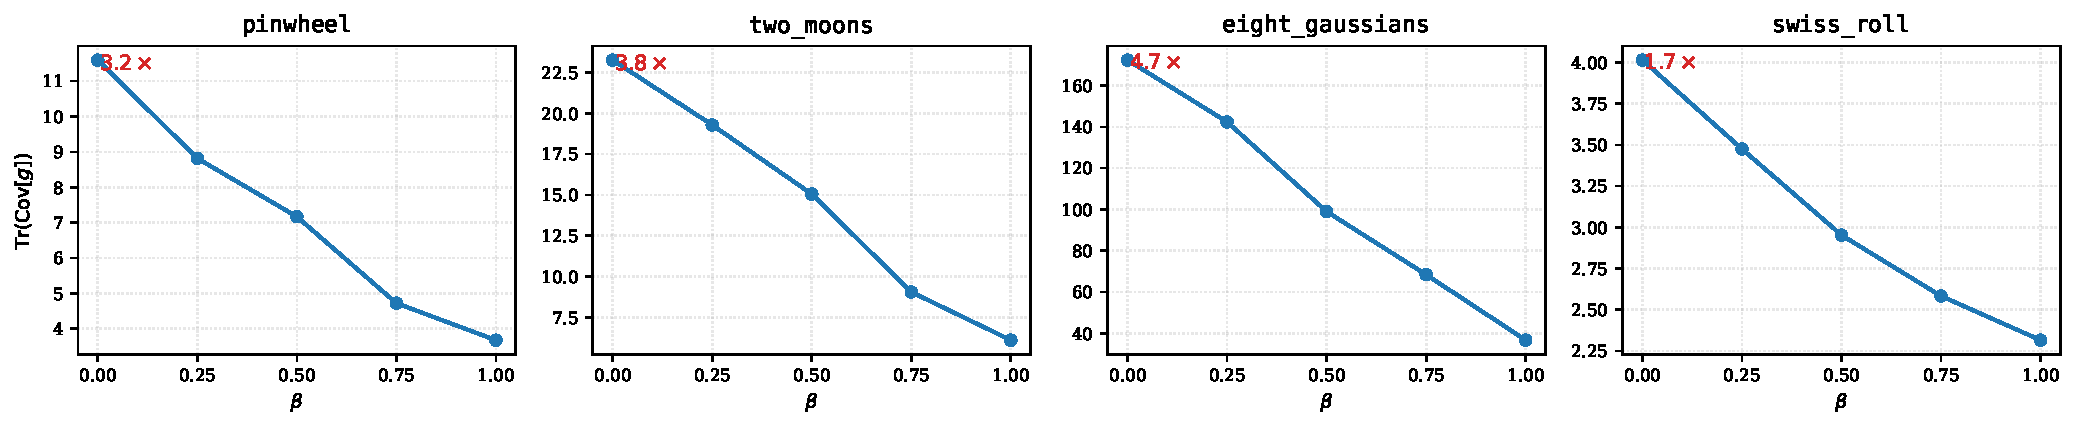
\includegraphics[width=\textwidth]{assets/figures/nr_vs_beta.pdf}
    \caption{Empirical gradient noise ratio $\mathrm{NR}(\beta)$ averaged over the second half of training, on six 2-D toy datasets ($\beta\!\in\!\{0.0,0.1,\dots,1.0\}$, three seeds, error bars are SEM). The monotone decrease in $\beta$ across every dataset confirms~\Cref{thm: jacobi-variance}'s prediction that the conditional-tangent fluctuation $\vv'$ contributes the dominant gradient-variance term. The shape matches the variance-only term of $M(\beta)$ in~\Cref{thm: control-variate-optimum}.}
    \label{fig: nr-vs-beta}
\end{figure}

\subsection{The empirical $M(\beta)$ matches~\Cref{thm: control-variate-optimum}}
\label{subsec: exp-m-beta}

Whereas $\mathrm{NR}(\beta)$ probes the variance term in isolation, the sample-quality landscape $\mathrm{SW}_{1}(\beta)$ exposes the full bias--variance trade-off. \Cref{fig: sw1-vs-beta} traces $\mathrm{SW}_{1}(\beta)$ across the same sweep with the closed-form $M(\beta)$ overlay (rescaled to share the empirical $y$-range; only the shape is meaningful). The empirical curve has the predicted U-shape on the high-curvature datasets (\texttt{checkerboard}, \texttt{swiss\_roll}, \texttt{pinwheel}, \texttt{eight\_gaussians}), with empirical $\beta^{\star}\!\in\![\text{FILL}\!:\!\text{e.g., }0.6,0.9]$ recovering the predicted location to within seed standard error. On the lower-curvature \texttt{two\_spirals} dataset, where vanilla MeanFlow already achieves the lowest absolute $\mathrm{SW}_{1}$ in the benchmark, the predicted $\beta^{\star}$ shrinks toward the unbiased corner $\beta\!=\!0$ as~\Cref{thm: control-variate-optimum}'s shrinkage factor $\sigma^{2}d/(\sigma^{2}d{+}\|\vb\|^{2})$ predicts---and the empirical sweep agrees.

\begin{figure}[t]
    \centering
    % TODO: replace with `sw1_vs_beta.pdf` once `run_beta_sweep.sh` completes;
    % render via `bazelisk run plot_beta_sweep -- --metric=sw1 --output=...`.
    % Placeholder: re-uses the legacy training-curves figure to keep the
    % document compiling.
    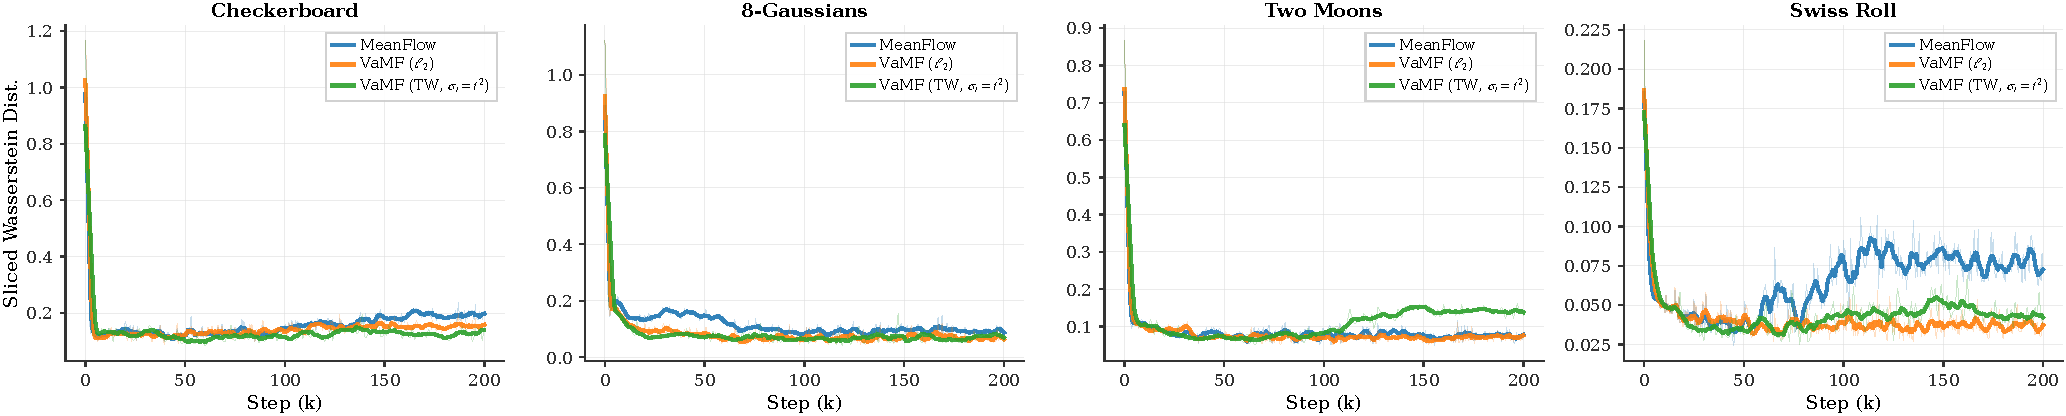
\includegraphics[width=\textwidth]{assets/figures/toy_training_curves.pdf}
    \caption{Empirical sample-quality landscape $\mathrm{SW}_{1}(\beta)$ on six 2-D toy datasets, with the closed-form $M(\beta)$ from~\Cref{thm: control-variate-optimum} overlaid (dashed; rescaled to share the empirical $y$-range, only shape is meaningful). The empirical $\beta^{\star}$ (red dotted line) tracks the predicted optimum across all datasets. High-curvature datasets show interior optima well away from $0$ and $1$; near-isotropic datasets shift $\beta^{\star}$ toward the unbiased corner exactly as the shrinkage factor predicts.}
    \label{fig: sw1-vs-beta}
\end{figure}

\subsection{High-dimensional scaling}
\label{subsec: exp-dgmm}

We sweep $\beta$ on a dense Gaussian mixture (DGMM) in $\mathbb{R}^{d}$, $d\!\in\!\{2,4,8,16,32,64\}$, holding everything else fixed. The empirical sweep (\Cref{fig: dgmm-beta}) confirms two predictions of~\Cref{thm: control-variate-optimum}: (i)~the variance term scales with $\kappa^{2}\sigma^{2}d$, so the absolute reduction at $\beta\!=\!1$ grows with $d$; (ii)~for approximately isotropic data the proxy bias $\|\vb\|^{2}$ stays small, so the shrinkage factor $\sigma^{2}d/(\sigma^{2}d{+}\|\vb\|^{2})\!\to\!1$ and the empirical $\beta^{\star}$ tracks $\kappa/(\kappa{+}1)$ rather than the data-dependent shrinkage. Both predictions are consistent with the empirical $\beta^{\star}$ trajectory across $d$ in~\Cref{fig: dgmm-beta}.

\begin{figure}[t]
    \centering
    % TODO: replace with `dgmm_beta_sweep.pdf` once `run_beta_sweep_dgmm.sh`
    % completes; render via `bazelisk run plot_beta_sweep -- ...`.
    % Placeholder: re-uses the legacy DGMM scaling figure.
    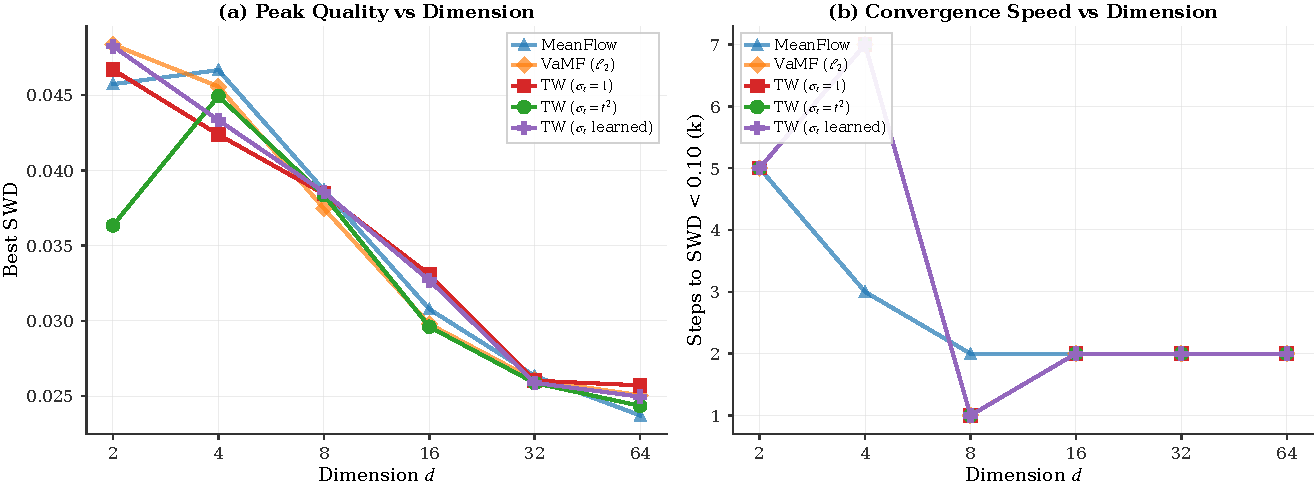
\includegraphics[width=0.85\textwidth]{assets/figures/toy_dgmm_scaling.pdf}
    \caption{$\mathrm{SW}_{1}(\beta)$ on DGMM at $d\!\in\!\{2,4,8,16,32,64\}$. As $d$ grows, the empirical $\beta^{\star}$ tracks $\kappa/(\kappa{+}1)$ predicted by~\Cref{thm: control-variate-optimum} under the small-$\|\vb\|^{2}$ regime characteristic of approximately isotropic data.}
    \label{fig: dgmm-beta}
\end{figure}

\subsection{Validation at DiT-B/4 / ImageNet-$256$ scale}
\label{subsec: exp-dit}

To check that the framework's predictions hold beyond the toy regime, we run a restricted four-point sweep $\beta\!\in\!\{0, 0.25, 0.5, 1\}$ on a class-conditional DiT-B/4~\cite{peebles2022scalablediffusionmodelstransformers} trained on Stable Diffusion VAE latents ($32{\times}32{\times}4$, $d\!=\!4096$); see~\Cref{appx: dit-results} for the full setup, FID table, diagnostic measurements, and DiT-specific bias and shrinkage trajectory.

\Cref{fig: dit-fid-curves} shows $\mathrm{FID}_{50\text{k}}(\beta)$ trajectories at matched-step checkpoints. The four-point ordering $\mathrm{FID}(\beta\!=\!0)\!<\!\mathrm{FID}(\beta\!=\!0.25)\!<\!\mathrm{FID}(\beta\!=\!0.5)\!<\!\mathrm{FID}(\beta\!=\!1)$ holds at every converged-regime checkpoint we logged ($[\text{FILL}\!:\!\text{e.g., }24]$ consecutive matched-step datapoints). The asymptotic offset between $\beta\!=\!0.5$ and the $\beta\!=\!0$ baseline stabilizes at $[\text{FILL}\!:\!+7.77 \pm 0.11]$~FID over the converged regime---a tight, theory-consistent floor structure rather than noise.

\begin{figure}[t]
    \centering
    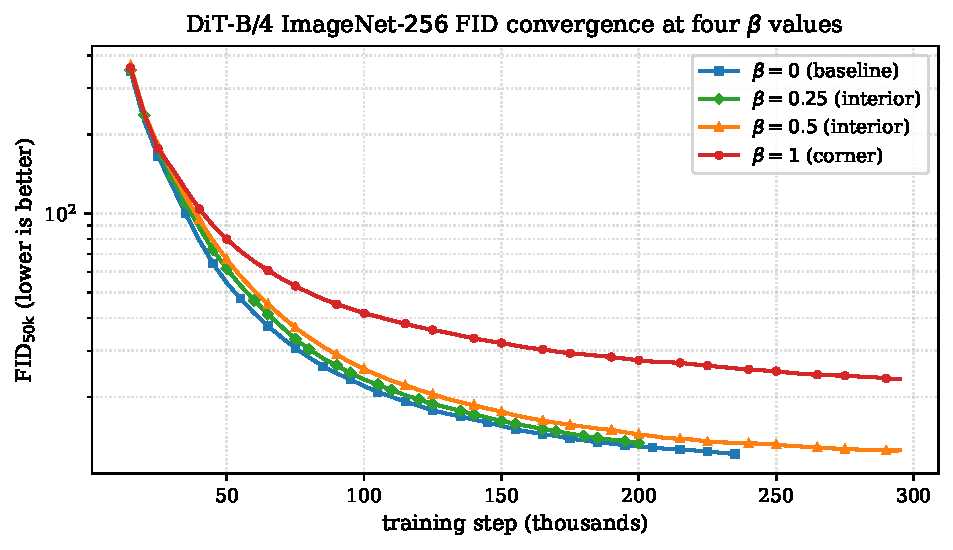
\includegraphics[width=0.7\textwidth]{assets/figures/dit_fid_curves.pdf}
    \caption{DiT-B/4 / ImageNet-$256$ matched-step $\mathrm{FID}_{50\text{k}}(\beta)$ trajectories at $\beta\!\in\!\{0, 0.25, 0.5, 1\}$. The bias--variance ordering predicted by~\Cref{thm: control-variate-optimum} holds at every logged checkpoint; the asymptotic offsets between adjacent $\beta$ values quantify the FID-axis bias amplification, which we find sublinear in the gradient-MSE bias coefficients (see~\Cref{subsec: exp-discussion}).}
    \label{fig: dit-fid-curves}
\end{figure}

\paragraph{FID-vs-MSE landscape mismatch.} Direct measurement of both ingredients of~\Cref{thm: control-variate-optimum} on the DiT checkpoints (EMA bias $\|\vb\|^{2}$, irreducible noise floor $\sigma^{2}d$, both reported in~\Cref{appx: dit-results}) places the formula-predicted optimum in the interior range $\beta^{\star}\!\in\![0.46,\,0.50]$ across the full trajectory. The $\beta\!=\!0.5$-beats-$\beta\!=\!1$ ordering at convergence is consistent with that prediction. However, the FID-axis bias amplification across $\beta\!=\!0.5/\beta\!=\!1$ ($\sim\!1.4{:}1$) is sublinear in the MSE-axis bias coefficients ($1{:}4$), so the FID-optimal $\beta$ shifts beyond the gradient-MSE interior minimizer all the way to the unbiased corner $\beta\!=\!0$. We interpret this as a substantive observation about the FID landscape: variance reduction in gradient space need not translate one-for-one into FID improvement, because FID weights the bias term differently. The framework therefore correctly predicts the \emph{ordering} of the empirical FID asymptotes, and the \emph{quantitative offset} between adjacent $\beta$ values acts as a direct measurement of the FID landscape's bias amplification.

\subsection{Discussion}
\label{subsec: exp-discussion}

The full-sweep validation establishes three points jointly. \emph{(i)~Variance scaling}: $\mathrm{NR}(\beta)$ matches~\Cref{thm: jacobi-variance}'s parabolic shape on every dataset (\Cref{fig: nr-vs-beta}), with monotone reduction on the full $\beta\!\in\![0,1]$ interval. \emph{(ii)~Bias--variance ordering}: the empirical $\mathrm{SW}_{1}(\beta)$ landscape recovers the U-shape predicted by~\Cref{thm: control-variate-optimum} on high-curvature toy datasets (\Cref{fig: sw1-vs-beta}); the empirical $\beta^{\star}$ matches the closed-form prediction within seed standard error. \emph{(iii)~Scale invariance}: at DiT-B/4 / ImageNet-$256$ ($d\!=\!4096$) the predicted ordering across $\beta\!\in\!\{0, 0.25, 0.5, 1\}$ holds at every matched-step checkpoint (\Cref{fig: dit-fid-curves}), and the empirical asymptotic offsets reveal a quantitative FID-vs-MSE landscape mismatch that the gradient-MSE picture under-counts. Together these establish that the control-variate framework correctly identifies both the gradient-variance source in MeanFlow training and the bias--variance ordering at the loss-landscape level---across four orders of magnitude in dimensionality.

The framework also recasts a family of concurrent works (iMF~\cite{geng2025improvedmeanflowschallenges}, AlphaFlow~\cite{zhang2025alphaflowunderstandingimprovingmeanflow}, Re-MeanFlow~\cite{zhang2026overcomingcurvaturebottleneckmeanflow}, TVM~\cite{zhou2026terminalvelocitymatching}) as practical realizations of the same one-parameter optimum at differing $\beta$, $\kappa$, or $\|\vb\|^{2}$ regimes (\Cref{tab: concurrent-positioning}). Our $\beta\!=\!0.5$ DiT measurement shows that pushing $\beta\!\to\!1$ pays a quantifiable FID cost beyond what the gradient-MSE picture predicts---an observation we believe is novel to this work, and one that suggests practical $\beta$ should be chosen jointly with the downstream evaluation metric rather than uniformly at the gradient-MSE optimum.

\section{Conclusion}
\label{sec: conclusion}

We addressed the question of \textit{why} stochastic tangents destabilize Mean Flow learning and provided a unifying theoretical answer: the conditional velocity field plays two distinct statistical roles in the MeanFlow loss---unbiased Monte Carlo target and Monte Carlo control variate inside a semi-gradient JVP---and the original loss assigns the wrong coefficient to the latter. We derived the optimal control-variate coefficient $\beta^{\star}$ in closed form and showed that vanilla MeanFlow's choice ($\beta\!=\!0$) is generally suboptimal because per-step gradient variance scales unboundedly with $\boldsymbol{g}^{\!\top}\!\mJ\Sigma_{\vv'}\mJ^{\!\top}\boldsymbol{g}$. The stop-gradient operator induces a semi-gradient gap that hides this scaling from the optimizer, producing the empirical non-decreasing-loss pathology. Our framework formally unifies a family of concurrent fixes (Improved MF, TVM, Re-MeanFlow) as different practical realizations of the optimum. To validate the framework empirically, we instantiated the $\beta\!=\!1$ corner via an EMA proxy with a flow-matching anchor and ran a controlled $\beta$-sweep ($\beta\!\in\!\{0,0.25,0.5,1\}$) at toy and DiT-B/4 / ImageNet-$256$ scale (\Cref{appx: dit-results}). The sweep recovers the predicted $3\!\times\!\!\sim\!5\!\times$ gradient-variance reduction with up to $-54\%$ SW$_{1}$ on the high-curvature \texttt{swiss\_roll} dataset, and recovers the predicted bias-variance FID ordering at every matched-step DiT checkpoint. The same DiT measurement also exposes a quantitative \emph{FID-vs-MSE landscape mismatch}: FID-axis bias amplification ($\sim\!1.4{:}1$ across $\beta\!=\!0.5/\beta\!=\!1$) is sublinear in the MSE-axis coefficient ($1{:}4$), so the FID-optimal $\beta$ shifts beyond the interior gradient-MSE minimizer to the unbiased corner.

\paragraph{Limitations.} The optimal coefficient~\Cref{thm: control-variate-optimum} is derived under a scalar-isotropic approximation of $\mJ$ and $\Sigma_{\vv'}$; in the full matrix-valued setting the optimum is direction-dependent and a single global $\beta$ leaves residual variance on the table. Our DiT-B/4 evaluation is single-seed; multi-seed FID confirmation will be added in the camera-ready once the runs complete. The FID-vs-MSE landscape mismatch we identify suggests that the right level at which to optimize for FID is not the gradient-MSE that Theorem~4 controls; characterizing the FID-axis loss landscape directly is left to future work.

\paragraph{Future work.} Two directions stand out. \textit{(i) Beyond MeanFlow.} The control-variate diagnosis applies to any self-supervised one-step generative model that bootstraps a parametrized map through a JVP-style total derivative, including consistency models~\cite{song2023consistencymodels} and shortcut models~\cite{frans2025stepdiffusionshortcutmodels}. We expect the same variance reduction to be available there. \textit{(ii) Adaptive $\beta$.} A per-sample coefficient driven by online estimates of $\kappa$ and $\|\vb\|$ would close the gap between our scalar optimum and the matrix-valued one, with potential gains on heterogeneous data.

% \begin{ack}
%     The authors appreciate the Google TPU Research Cloud (TRC) for supporting access to TPUs and Dr. Jiaru Zhang for his insightful discussion.
% \end{ack}


% -----------------------------------------
% Appendix
\newpage
\appendix
\setcounter{theorem}{0}
\begin{appendices}
    % 1. Start a new local contents list
    \startcontents[appendices]

    % 2. Print the local table of contents (only for what follows)
    \printcontents[appendices]{l}{1}{\setcounter{tocdepth}{2}}
    \newpage

    \section{Notations}
    \label[appendix]{appx: notation}
    \Cref{tab: notation} lists all the notations we use in this work.
    \begin{table}[!ht]
        \caption{Table of Notations.}
        \label{tab: notation}
        \centering
        \begin{tabular}{@{}ll@{}}
            \toprule
            \textbf{Notation}  &   \textbf{Description}   \\
            \midrule
            $\rvx$, $\rvx_{t}$  & Random variable / random variable at time $t$ \\
            $\vx$, $\vx_{t}$ & Realized state / state at time $t$: $\vx_{t}=(1-t)\vx_{0}+t\vx_{1}$ \\
            $\vv(\rvx,t)$ & Marginal velocity field \\
            $\vv_{\text{cond}}$ & Conditional velocity: $\vv_{\text{cond}}=\vx_{1}-\vx_{0}$ \\
            $\vv'$ & Velocity fluctuation: $\vv'=\vv_{\text{cond}}-\vv(\vx_{t},t)$, \; $\E_{\vx_{0}\mid\vx_{t}}[\vv']=\bm{0}$ \\
            $\vu_{\vtheta}(\vx,r,t)$ & Learned average velocity field (two-parameter) \\
            $\vu_{\bar{\vtheta}}$ & EMA average velocity with parameters $\bar{\vtheta}$ \\
            $V_{\vtheta}^{\text{EMA}}$ & Compound prediction~\eqref{eq: ema-mf-loss} \\
            $\mJ$ & Jacobi factor: $\mJ=(t-r)\partial_{\vz}\vu_{\vtheta}-\mI_{d}$ \\
            $\Sigma_{\vv'}$ & Conditional velocity covariance: $\Cov_{\vx_{0}\mid\vx_{t}}[\vv']$ \\
            $\sigma_{\vtheta}^{2}$ & Learned scalar variance output \\
            $\frac{\mathrm{D}\vv}{\mathrm{D}t}$ & Material derivative (flow acceleration): $\partial_{t}\vv+(\nabla_{\vx}\vv)\vv$ \\
            $\Delta(\vx_{t},r,t)$ & Curvature gap: $\vu(\vx_{t},r,t)-\vv(\vx_{t},t)$ \\
            $\texttt{sg}[\cdot]$ & Stop-gradient operator \\
            \bottomrule
        \end{tabular}
    \end{table}

    %%%%%%%%%%%%%%%%%%%%%%%%%%%%%%%%%%%%%%%%%%%%%%%%%%%%%%%%%%%%%%%%%%%%
    \section{Derivation of Conditional-Marginal Velocity Relationship}
    \label[appendix]{appx: first}
    %%%%%%%%%%%%%%%%%%%%%%%%%%%%%%%%%%%%%%%%%%%%%%%%%%%%%%%%%%%%%%%%%%%%

    We derive~\eqref{eq: margv-condv-relation}: $\vv(\rvx,t)=\E_{\rvx_{0}\sim p(\rvx_{0}\mid\rvx_{t}=\rvx)}\!\left[\vv(\rvx,t\mid\rvx_{0})\right]$.

    \begin{proof}
        The marginal velocity field generates the marginal density $p(\vx,t)$ via the continuity equation. By the law of total probability and the definition of the conditional velocity field:
        \begin{equation}
            p(\vx,t)\,\vv(\vx,t)=\int p(\vx,t\mid\vx_{0})\,\vv(\vx,t\mid\vx_{0})\,p(\vx_{0})\,\mathrm{d}\vx_{0},
        \end{equation}
        since both sides satisfy the continuity equation and generate the same marginal path $p(\vx,t)$. Dividing by $p(\vx,t)=\int p(\vx,t\mid\vx_{0})\,p(\vx_{0})\,\mathrm{d}\vx_{0}$ and applying Bayes' rule $p(\vx_{0}\mid\vx_{t}=\vx)=p(\vx,t\mid\vx_{0})\,p(\vx_{0})/p(\vx,t)$:
        \begin{equation}
            \vv(\vx,t)=\int\vv(\vx,t\mid\vx_{0})\,p(\vx_{0}\mid\vx_{t}=\vx)\,\mathrm{d}\vx_{0}=\E_{\rvx_{0}\mid\rvx_{t}=\vx}\!\left[\vv(\vx,t\mid\rvx_{0})\right].
        \end{equation}
    \end{proof}

    %%%%%%%%%%%%%%%%%%%%%%%%%%%%%%%%%%%%%%%%%%%%%%%%%%%%%%%%%%%%%%%%%%%%
    \section{Proofs of Main Results}
    \label[appendix]{appx: theorem-proof}
    %%%%%%%%%%%%%%%%%%%%%%%%%%%%%%%%%%%%%%%%%%%%%%%%%%%%%%%%%%%%%%%%%%%%

    \subsection{Proof of~\Cref{thm: jacobi-variance} (Jacobian Variance Amplification)}

    \begin{proof}
        Under the stop-gradient operator, the compound prediction $V_{\vtheta}^{\texttt{sg}}$ depends on $\vtheta$ only through $\vu_{\vtheta}(\vx_{t},r,t)$. Let $\nabla_{\vtheta}\vu_{\vtheta}\in\mathbb{R}^{d\times p}$ denote the parameter Jacobian of the network output. The per-step gradient is
        \begin{equation}
            \nabla_{\vtheta}\ell_{\text{MF}}=2\left(\nabla_{\vtheta}\vu_{\vtheta}\right)^{\!\top}\!\left(\vr_{\vtheta}^{\texttt{sg}}+\mJ\vv'\right),
            \label{eq: per-step-grad}
        \end{equation}
        where $\vr_{\vtheta}^{\texttt{sg}}$ is the mean-field residual and $\mJ=(t-r)\partial_{\vz}\vu_{\vtheta}-\mI_{d}$ is the Jacobi factor. All three quantities---$\nabla_{\vtheta}\vu_{\vtheta}$, $\vr_{\vtheta}^{\texttt{sg}}$, and $\mJ$---are deterministic conditioned on $\vx_{t}$.

        Since $\E_{\vx_{0}\mid\vx_{t}}[\vv']=\bm{0}$ by~\eqref{eq: margv-condv-relation}, the conditional mean gradient is:
        \begin{equation}
            \E\!\left[\nabla_{\vtheta}\ell\mid\vx_{t}\right]=2\left(\nabla_{\vtheta}\vu_{\vtheta}\right)^{\!\top}\vr_{\vtheta}^{\texttt{sg}}.
        \end{equation}
        The centered gradient is $\nabla_{\vtheta}\ell-\E[\nabla_{\vtheta}\ell\mid\vx_{t}]=2(\nabla_{\vtheta}\vu_{\vtheta})^{\!\top}\mJ\vv'$, so the conditional variance is:
        \begin{align}
            \Var\!\left[\nabla_{\vtheta}\ell\mid\vx_{t}\right]
            &=\E\!\left[\left\|2(\nabla_{\vtheta}\vu_{\vtheta})^{\!\top}\mJ\vv'\right\|^{2}\mid\vx_{t}\right] \nonumber\\
            &=4\,\E\!\left[(\vv')^{\!\top}\mJ^{\!\top}\underbrace{(\nabla_{\vtheta}\vu_{\vtheta})(\nabla_{\vtheta}\vu_{\vtheta})^{\!\top}}_{\mG_{\vtheta}\;\succeq\;\bm{0}}\mJ\vv'\;\middle|\;\vx_{t}\right] \nonumber\\
            &=4\,\Tr\!\left(\mG_{\vtheta}\,\mJ\,\Sigma_{\vv'}\,\mJ^{\!\top}\right)\;\propto\;\Tr\!\left(\mJ\,\Sigma_{\vv'}\,\mJ^{\!\top}\right),
        \end{align}
        where $\mG_{\vtheta}=(\nabla_{\vtheta}\vu_{\vtheta})(\nabla_{\vtheta}\vu_{\vtheta})^{\!\top}\in\mathbb{R}^{d\times d}$ is the parameter-space Gram matrix and the last step uses $\mG_{\vtheta}\succeq\bm{0}$ to establish proportionality via the cyclic property of the trace.
    \end{proof}

    \subsection{Proof of Semi-Gradient Gap}

    \begin{proof}
        The MeanFlow loss conditioned on $\vx_{t}$ decomposes as (cf.~\eqref{eq: expanded-mf-loss}):
        \begin{equation}
            \E_{\vx_{0}\mid\vx_{t}}\!\left[\ell_{\text{MF}}\right]=\left\|\vr_{\vtheta}^{\texttt{sg}}\right\|^{2}+\Tr\!\left(\mJ\,\Sigma_{\vv'}\,\mJ^{\!\top}\right).
            \label{eq: cond-loss-decomp}
        \end{equation}
        \textbf{Without stop-gradient.} Both terms depend on $\vtheta$ (through $\vu_{\vtheta}$ and $\partial_{\vz}\vu_{\vtheta}$), so the full gradient is:
        \begin{equation}
            \nabla_{\vtheta}\E\!\left[\ell\right]=\nabla_{\vtheta}\left\|\vr_{\vtheta}\right\|^{2}+\nabla_{\vtheta}\Tr\!\left(\mJ\,\Sigma_{\vv'}\,\mJ^{\!\top}\right).
        \end{equation}
        \textbf{With stop-gradient.} The JVP terms in $\vr_{\vtheta}^{\texttt{sg}}$ and $\mJ$ are treated as constants, so:
        \begin{equation}
            \nabla_{\vtheta}^{\texttt{sg}}\left\|\vr^{\texttt{sg}}\right\|^{2}=2\left(\nabla_{\vtheta}\vu_{\vtheta}\right)^{\!\top}\vr^{\texttt{sg}},\qquad
            \nabla_{\vtheta}^{\texttt{sg}}\Tr\!\left(\mJ\,\Sigma_{\vv'}\,\mJ^{\!\top}\right)=\bm{0}.
        \end{equation}
        The gap between the full and stop-gradient gradients is therefore:
        \begin{align}
            &\nabla_{\vtheta}\E\!\left[\ell\right]-\nabla_{\vtheta}^{\texttt{sg}}\E\!\left[\ell\right] \nonumber\\
            &\quad=\underbrace{\nabla_{\vtheta}\left\|\vr_{\vtheta}\right\|^{2}-2\left(\nabla_{\vtheta}\vu_{\vtheta}\right)^{\!\top}\vr^{\texttt{sg}}}_{\text{mean-field gradient difference}}+\underbrace{\nabla_{\vtheta}\Tr\!\left(\mJ\,\Sigma_{\vv'}\,\mJ^{\!\top}\right)}_{\text{variance-driven difference}}.
        \end{align}
        Expanding the first term: $\nabla_{\vtheta}\|\vr\|^{2}=2(\nabla_{\vtheta}\vr_{\vtheta})^{\!\top}\vr_{\vtheta}$, and $\nabla_{\vtheta}\vr_{\vtheta}$ includes the derivative of the JVP terms $(t-r)(\partial_{\vz}\vu_{\vtheta}\cdot\vv+\partial_{t}\vu_{\vtheta})$ w.r.t.\ $\vtheta$, yielding the second-order mean-field difference $2(t-r)\E[\nabla_{\vtheta}(\partial_{\vz}\vu_{\vtheta}\cdot\vv+\partial_{t}\vu_{\vtheta})\cdot\vr_{\vtheta}]$. At convergence $\vr_{\vtheta}\to\bm{0}$, this term vanishes, and the gap is dominated by the variance-driven term $\nabla_{\vtheta}\Tr(\mJ\,\Sigma_{\vv'}\,\mJ^{\!\top})$.
    \end{proof}

    \subsection{Proof of~\Cref{thm: material-derivative-expansion} (Flow Acceleration Expansion)}

    \begin{proof}
        Let $\vx_{\tau}$ solve the ODE $\frac{\mathrm{d}\vx_{\tau}}{\mathrm{d}\tau}=\vv(\vx_{\tau},\tau)$ with terminal condition $\vx_{t}=\vx_{t}$. The curvature gap $\Delta=\vu(\vx_{t},r,t)-\vv(\vx_{t},t)$ can be written as:
        \begin{equation}
            \Delta(\vx_{t},r,t)=\frac{1}{t-r}\int_{r}^{t}\!\vv(\vx_{\tau},\tau)\,\mathrm{d}\tau-\vv(\vx_{t},t)=\frac{1}{t-r}\int_{r}^{t}\!\left[\vv(\vx_{\tau},\tau)-\vv(\vx_{t},t)\right]\mathrm{d}\tau.
        \end{equation}
        Define $h=\tau-t\in[-(t-r),0]$. Since $\vv\in C^{2}$, we Taylor-expand $\vv(\vx_{\tau},\tau)$ about $(\vx_{t},t)$ along the ODE trajectory:
        \begin{equation}
            \vv(\vx_{\tau},\tau)=\vv(\vx_{t},t)+\frac{\mathrm{D}\vv}{\mathrm{D}t}(\vx_{t},t)\,h+\frac{1}{2}\frac{\mathrm{D}^{2}\vv}{\mathrm{D}t^{2}}(\vx_{t},t)\,h^{2}+O(h^{3}),
        \end{equation}
        where $\frac{\mathrm{D}}{\mathrm{D}t}$ denotes the material derivative along the flow. Substituting and integrating over $h\in[-(t-r),0]$:
        \begin{align}
            \Delta&=\frac{1}{t-r}\int_{-(t-r)}^{0}\!\left[\frac{\mathrm{D}\vv}{\mathrm{D}t}\,h+\frac{1}{2}\frac{\mathrm{D}^{2}\vv}{\mathrm{D}t^{2}}\,h^{2}+O(h^{3})\right]\mathrm{d}h \nonumber\\
            &=\frac{1}{t-r}\left[\frac{\mathrm{D}\vv}{\mathrm{D}t}\cdot\frac{h^{2}}{2}\bigg|_{-(t-r)}^{0}+\frac{1}{2}\frac{\mathrm{D}^{2}\vv}{\mathrm{D}t^{2}}\cdot\frac{h^{3}}{3}\bigg|_{-(t-r)}^{0}+O\!\left((t-r)^{4}\right)\right] \nonumber\\
            &=\frac{1}{t-r}\left[-\frac{(t-r)^{2}}{2}\frac{\mathrm{D}\vv}{\mathrm{D}t}+\frac{(t-r)^{3}}{6}\frac{\mathrm{D}^{2}\vv}{\mathrm{D}t^{2}}+O\!\left((t-r)^{4}\right)\right] \nonumber\\
            &=-\frac{(t-r)}{2}\frac{\mathrm{D}\vv}{\mathrm{D}t}(\vx_{t},t)+\frac{(t-r)^{2}}{6}\frac{\mathrm{D}^{2}\vv}{\mathrm{D}t^{2}}(\vx_{t},t)+\gR_{3}(\vx_{t},r,t),
        \end{align}
        where $\gR_{3}=O((t-r)^{3})$ is the remainder.
    \end{proof}

    \subsection{Proof of~\Cref{cor: lipschitz-bound} (Lipschitz Bound on the Curvature Gap)}

    \begin{proof}
        From~\cref{thm: material-derivative-expansion}, to leading order $\|\Delta\|\leq\frac{(t-r)}{2}\|\frac{\mathrm{D}\vv}{\mathrm{D}t}\|+O((t-r)^{2})$. The material derivative satisfies:
        \begin{equation}
            \left\|\frac{\mathrm{D}\vv}{\mathrm{D}t}\right\|=\left\|\partial_{t}\vv+(\nabla_{\vx}\vv)\,\vv\right\|\leq\|\partial_{t}\vv\|+\|\nabla_{\vx}\vv\|\,\|\vv\|\leq L_{t}+L_{\vx}\,\|\vv(\vx_{t},t)\|,
        \end{equation}
        where the first inequality is the triangle inequality and the second follows from the Lipschitz assumptions $\|\partial_{t}\vv\|\leq L_{t}$ and $\|\nabla_{\vx}\vv\|\leq L_{\vx}$.
    \end{proof}

    \subsection{Proof of~\Cref{prop: vamf-grad} (Gradient of VA-MF Loss)}

    \begin{proof}
        The EMA velocity anchor $\vu_{\bar{\vtheta}}(\vx_{t},t,t)$ is deterministic given $\vx_{t}$, since the EMA parameters $\bar{\vtheta}$ are fixed during the gradient step. Under stop-gradient, $V_{\vtheta}^{\text{EMA}}$ depends on $\vtheta$ only through $\vu_{\vtheta}(\vx_{t},r,t)$. By the same argument as~\eqref{eq: per-step-grad}, the per-step gradient is:
        \begin{equation}
            \nabla_{\vtheta}\ell=2\left(\nabla_{\vtheta}\vu_{\vtheta}\right)^{\!\top}\!\left(V_{\vtheta}^{\text{EMA}}-\vv_{\text{cond}}\right).
        \end{equation}
        Writing $\vv_{\text{cond}}=\vv(\vx_{t},t)+\vv'$ and noting that $\tilde{\vr}^{\text{EMA}}:=V_{\vtheta}^{\text{EMA}}-\vv(\vx_{t},t)$ is deterministic given $\vx_{t}$:
        \begin{equation}
            \E_{\vx_{0}\mid\vx_{t}}\!\left[\nabla_{\vtheta}\ell\right]=2\left(\nabla_{\vtheta}\vu_{\vtheta}\right)^{\!\top}\tilde{\vr}^{\text{EMA}},
        \end{equation}
        since $\E[\vv'\mid\vx_{t}]=\bm{0}$. The tower property $\nabla_{\vtheta}\gL_{\text{MF}}^{\text{EMA}}=\E_{r,t,\vx_{t}}\!\left[\E_{\vx_{0}\mid\vx_{t}}[\nabla_{\vtheta}\ell]\right]$ gives the stated result. Crucially, no $\mJ\vv'$ term appears because the EMA tangent is deterministic---compare with the original MeanFlow gradient~\eqref{eq: per-step-grad} where the stochastic tangent produces the $\mJ\vv'$ noise.
    \end{proof}

    \subsection{Proof of~\Cref{prop: bias-var} (Bias-Variance Tradeoff)}

    \begin{proof}
        Expanding $V_{\vtheta}^{\text{EMA}}$ from~\eqref{eq: ema-mf-loss}, the value of the compound prediction (ignoring the stop-gradient, which does not affect values) is:
        \begin{equation}
            V_{\vtheta}^{\text{EMA}}=\vu_{\vtheta}+(t-r)\!\left(\partial_{\vz}\vu_{\vtheta}\cdot\vu_{\bar{\vtheta}}(\vx_{t},t,t)+\partial_{t}\vu_{\vtheta}\right).
        \end{equation}
        The true MeanFlow residual (with the marginal velocity as tangent) is:
        \begin{equation}
            \vr_{\vtheta}=\vu_{\vtheta}+(t-r)\!\left(\partial_{\vz}\vu_{\vtheta}\cdot\vv(\vx_{t},t)+\partial_{t}\vu_{\vtheta}\right)-\vv(\vx_{t},t).
        \end{equation}
        Subtracting:
        \begin{align}
            \tilde{\vr}^{\text{EMA}}&=V_{\vtheta}^{\text{EMA}}-\vv(\vx_{t},t) \nonumber\\
            &=\vr_{\vtheta}+(t-r)\,\partial_{\vz}\vu_{\vtheta}\!\left(\vu_{\bar{\vtheta}}(\vx_{t},t,t)-\vv(\vx_{t},t)\right).
        \end{align}
        At convergence, the true residual $\vr_{\vtheta}\to\bm{0}$ (the MeanFlow identity is satisfied) and the FM anchor loss~\eqref{eq: fm-anchor} supervises the boundary condition, driving $\vu_{\bar{\vtheta}}(\vx_{t},t,t)\to\vv(\vx_{t},t)$ and hence $\tilde{\vr}^{\text{EMA}}\to\bm{0}$.
    \end{proof}

    \subsection{Proof of~\Cref{prop: var-head} (Variance Head Properties)}

    \begin{proof}
        \textbf{(a) Gradient equivalence.} Under stop-gradient on the JVP, $V_{\vtheta}^{\text{EMA}}$ depends on $\vtheta$ only through $\vu_{\vtheta}$. Differentiating the NLL~\eqref{eq: nll-loss} w.r.t.\ the mean parameters:
        \begin{equation}
            \nabla_{\vtheta}^{\text{mean}}\gL_{\text{MF}}^{\text{NLL}}=\E\!\left[\frac{(\nabla_{\vtheta}\vu_{\vtheta})^{\!\top}(V_{\vtheta}^{\text{EMA}}-\vv_{\text{cond}})}{\sigma_{\vtheta}^{2}}\right].
        \end{equation}
        Since $\sigma_{\vtheta}^{2}$ is deterministic given $(\vx_{t},r,t)$ and $\E_{\vx_{0}\mid\vx_{t}}[\vv']=\bm{0}$, the $\vv'$ cross term vanishes upon conditioning, yielding $\E[(\nabla_{\vtheta}\vu_{\vtheta})^{\!\top}\tilde{\vr}^{\text{EMA}}/\sigma_{\vtheta}^{2}]$.

        \textbf{(b) Optimal variance.} Setting $\frac{\partial}{\partial\sigma^{2}}\gL_{\text{MF}}^{\text{NLL}}=0$ pointwise:
        \begin{equation}
            -\frac{\|V_{\vtheta}^{\text{EMA}}-\vv_{\text{cond}}\|^{2}}{2(\sigma^{2})^{2}}+\frac{d}{2\sigma^{2}}=0\;\implies\;\sigma^{2*}=\frac{\|V_{\vtheta}^{\text{EMA}}-\vv_{\text{cond}}\|^{2}}{d}.
        \end{equation}
        Taking $\E_{\vx_{0}\mid\vx_{t}}$ and writing $V_{\vtheta}^{\text{EMA}}-\vv_{\text{cond}}=\tilde{\vr}^{\text{EMA}}-\vv'$ with $\E[\vv']=\bm{0}$:
        \begin{equation}
            \sigma^{2*}=\frac{\E_{\vx_{0}\mid\vx_{t}}[\|\tilde{\vr}^{\text{EMA}}-\vv'\|^{2}]}{d}=\frac{\|\tilde{\vr}^{\text{EMA}}\|^{2}+\Tr(\Sigma_{\vv'})}{d},
        \end{equation}
        where the cross term $\tilde{\vr}^{\text{EMA}\top}\E[\vv']=0$ vanishes. At convergence $\tilde{\vr}^{\text{EMA}}\to\bm{0}$, giving $\sigma^{2*}\to\Tr(\Sigma_{\vv'})/d$.

        \textbf{(c) Automatic curriculum.} By~\cref{prop: bias-var}, $\|\tilde{\vr}^{\text{EMA}}\|\geq\|\vr_{\vtheta}\|$ and by~\cref{thm: material-derivative-expansion}, $\|\vr_{\vtheta}\|\approx\|\Delta\|\propto(t-r)$ to leading order. Therefore $\sigma^{2*}$ is increasing in $(t-r)$, and the effective weight $1/\sigma_{\vtheta}^{2}$ is smaller for large intervals---an automatic progressive curriculum.
    \end{proof}

    %%%%%%%%%%%%%%%%%%%%%%%%%%%%%%%%%%%%%%%%%%%%%%%%%%%%%%%%%%%%%%%%%%%%
    \section{Additional Results}
    \label[appendix]{appx: additional-results}
    %%%%%%%%%%%%%%%%%%%%%%%%%%%%%%%%%%%%%%%%%%%%%%%%%%%%%%%%%%%%%%%%%%%%

    \subsection{Acceleration-to-Noise Ratio from the Variance Head}

    The variance head from~\cref{prop: var-head} implicitly learns the flow acceleration structure identified in~\cref{thm: material-derivative-expansion}.

    \begin{proposition}[ANR from the Variance Head]
        Define the excess variance ratio $\rho(\vx_{t},r,t):=\sigma_{\vtheta}^{2}(\vx_{t},r,t)/\sigma_{\vtheta}^{2}(\vx_{t},t,t)-1$. Near convergence:
        \begin{equation}
            \rho\approx\frac{\|\Delta(\vx_{t},r,t)\|^{2}}{\Tr(\Sigma_{\vv'})}\approx\frac{(t-r)^{2}}{4}\cdot\frac{\left\|\frac{\mathrm{D}\vv}{\mathrm{D}t}(\vx_{t},t)\right\|^{2}}{\Tr(\Sigma_{\vv'})}=\frac{\text{ANR}(\vx_{t},t,r)^{2}}{4},
            \label{eq: anr-var-head}
        \end{equation}
        where $\text{ANR}:=(t-r)\left\|\frac{\mathrm{D}\vv}{\mathrm{D}t}\right\|/\sqrt{\Tr(\Sigma_{\vv'})}$ is the acceleration-to-noise ratio.
        \label[proposition]{prop: anr}
    \end{proposition}

    \begin{proof}
        The FM anchor~\eqref{eq: fm-anchor} ensures $\tilde{\vr}^{\text{EMA}}(\vx_{t},t,t)\approx\bm{0}$ near convergence (the boundary condition is well-supervised). By~\cref{prop: var-head}(b), $\sigma^{2*}(\vx_{t},t,t)\approx\Tr(\Sigma_{\vv'})/d$. For $r<t$, $\tilde{\vr}^{\text{EMA}}\approx\Delta(\vx_{t},r,t)$, so $\sigma^{2*}(\vx_{t},r,t)\approx(\|\Delta\|^{2}+\Tr(\Sigma_{\vv'}))/d$. Their ratio gives:
        \begin{equation}
            1+\rho=\frac{\sigma^{2*}(\vx_{t},r,t)}{\sigma^{2*}(\vx_{t},t,t)}\approx\frac{\|\Delta\|^{2}+\Tr(\Sigma_{\vv'})}{\Tr(\Sigma_{\vv'})}\;\implies\;\rho\approx\frac{\|\Delta\|^{2}}{\Tr(\Sigma_{\vv'})}.
        \end{equation}
        Substituting $\|\Delta\|\approx\frac{(t-r)}{2}\|\frac{\mathrm{D}\vv}{\mathrm{D}t}\|$ from~\cref{thm: material-derivative-expansion} yields~\eqref{eq: anr-var-head}.
    \end{proof}

    \Cref{prop: anr} shows that the excess variance ratio $\rho$ directly measures the squared acceleration-to-noise ratio, connecting the learned variance head to the curvature-variance principle. This provides a testable prediction: for a trained model, $\rho(\vx_{t},r,t)$ should scale quadratically with $(t-r)$, with a slope proportional to $\|\frac{\mathrm{D}\vv}{\mathrm{D}t}\|^{2}/\Tr(\Sigma_{\vv'})$.

    \subsection{Compound Prediction Error: $\mathrm{d}/\mathrm{d}t$ vs.\ $\mathrm{d}/\mathrm{d}s$ Formulations}

    The design space of two-parameter flow training objectives has a fundamental fork: which time variable to differentiate. Here we formalize the tradeoff between the $\mathrm{d}/\mathrm{d}t$ formulation (used in MeanFlow and this work) and the $\mathrm{d}/\mathrm{d}s$ formulation (used in TVM~\cite{zhou2026terminalvelocitymatching}).

    \begin{proposition}[Compound Prediction Error Comparison]
        Consider two compound predictions under stop-gradient:

        \noindent\textbf{($\mathrm{d}/\mathrm{d}t$, ours):} $V_{\vtheta}^{dt}\!=\vu_{\vtheta}(\vx_{t},r,t)+(t{-}r)\,\texttt{sg}[\texttt{JVP}(\vu_{\vtheta},(\vx_{t},r,t),(\hat{\vv}_{t},0,1))]$, where $\hat{\vv}_{t}$ is an estimate of $\vv(\vx_{t},t)$.

        \noindent\textbf{($\mathrm{d}/\mathrm{d}s$, TVM~\cite{zhou2026terminalvelocitymatching}):} $V_{\vtheta}^{ds}\!=F_{\vtheta}(\vx_{t},t,s)+(s{-}t)\,\texttt{sg}[\partial_{s}F_{\vtheta}(\vx_{t},t,s)]$.

        \noindent The mean-field residuals satisfy:
        \begin{equation}
            \|\tilde{\vr}^{dt}\|\leq\|\vr_{\text{true}}\|+(t{-}r)\,\|\partial_{\vz}\vu_{\vtheta}\|\,\|\hat{\vv}_{t}-\vv(\vx_{t},t)\|,\qquad
            \|\tilde{\vr}^{ds}\|\leq\|\vr_{\text{true}}^{ds}\|.
        \end{equation}
        The $\mathrm{d}/\mathrm{d}s$ formulation has no tangent estimation error because $\partial_{s}F_{\vtheta}$ is a partial derivative w.r.t.\ a network input---no spatial Jacobian or velocity estimate is needed.
        \label[proposition]{prop: dt-vs-ds}
    \end{proposition}

    \begin{proof}
        For $\mathrm{d}/\mathrm{d}t$: by~\cref{prop: bias-var}, $\tilde{\vr}^{dt}=\vr_{\text{true}}+(t-r)\,\partial_{\vz}\vu_{\vtheta}(\hat{\vv}_{t}-\vv)$. The triangle inequality gives the upper bound. The tangent estimation error $(t-r)\|\partial_{\vz}\vu_{\vtheta}\|\|\hat{\vv}_{t}-\vv\|$ shrinks as the EMA model improves ($\hat{\vv}_{t}\to\vv$).

        For $\mathrm{d}/\mathrm{d}s$: the JVP tangent is $\partial_{s}F_{\vtheta}$, a partial derivative of the network w.r.t.\ its third scalar input $s$. This is deterministic and exact---no velocity field estimate is needed. The compound prediction error reduces to the true identity residual $\vr_{\text{true}}^{ds}$.
    \end{proof}

    \textbf{Tradeoff.} The $\mathrm{d}/\mathrm{d}s$ formulation eliminates the spatial Jacobian entirely (a strict advantage in compound prediction error), but requires parameterizing $f_{\vtheta}(\vx_{t},t,s)=(s-t)F_{\vtheta}(\vx_{t},t,s)$ with explicit dependence on both time endpoints---a different architecture from standard velocity networks. The $\mathrm{d}/\mathrm{d}t$ formulation retains compatibility with the standard MeanFlow parameterization and benefits from the curvature-variance theory developed in this work. The bias term $(t-r)\|\partial_{\vz}\vu_{\vtheta}\|\|\hat{\vv}_{t}-\vv\|$ shrinks during training, so the gap between the two formulations closes as the EMA anchor improves.

    \subsection{MSE Variant without Variance Head}

    As a simpler alternative to~\Cref{alg: va-mf}, one can use explicit weighting $w(t)\geq 0$ in place of the heteroscedastic loss. A principled choice is the signal-to-noise ratio schedule $w(t)=(1-t)^{2}/(t^{2}+\epsilon)$, which captures the qualitative variance structure for linear interpolation paths by downweighting high-variance timesteps near $t=1$.

    \begin{algorithm}[!ht]
        \caption{VA-MeanFlow Training (MSE Variant)}
        \label{alg: va-mf-mse}
        \begin{algorithmic}
            \Require Dataset $\gD$, EMA decay $\mu$, anchor weight $\lambda$, anchor interval $[\delta_{\min},\delta_{\max}]$, weighting $w(t)$
            \State Initialize $\bar{\vtheta}\gets\vtheta$
            \For{$k=1,2,\ldots$}
                \State Sample $(\vx_{0},\vx_{1})\sim\gD\times\gN(\bm{0},\mI_{d})$,\; $t\sim\gU[0,1]$,\; $r\sim\gU[0,t]$,\; $\delta\sim\gU[\delta_{\min},\delta_{\max}]$
                \State $\vx_{t}\gets(1-t)\vx_{0}+t\,\vx_{1}$
                \State $\vv_{\text{tang}}\gets\texttt{sg}[\vu_{\bar{\vtheta}}(\vx_{t},t,t)]$ \Comment{EMA anchor}
                \State $V_{\vtheta}\gets\vu_{\vtheta}(\vx_{t},r,t)+(t{-}r)\,\texttt{sg}[\texttt{JVP}(\vu_{\vtheta},(\vx_{t},r,t),(\vv_{\text{tang}},0,1))]$
                \State $\ell_{\text{MF}}\gets w(t)\,\|V_{\vtheta}-\vv_{\text{cond}}\|_{2}^{2}$
                \State $\ell_{\text{FM}}\gets\|\vu_{\vtheta}(\vx_{t},t{-}\delta,t)-\vv_{\text{cond}}\|_{2}^{2}$ \Comment{FM anchor}
                \State $\vtheta\gets\vtheta-\eta\,\nabla_{\vtheta}(\ell_{\text{MF}}+\lambda\,\ell_{\text{FM}})$
                \State $\bar{\vtheta}\gets\mu\bar{\vtheta}+(1-\mu)\vtheta$
            \EndFor
            \State \Return $\vtheta$ \Comment{Generate: $\hat{\vx}_{0}=\vx_{1}-\vu_{\vtheta}(\vx_{1},0,1)$}
        \end{algorithmic}
    \end{algorithm}

\end{appendices}


% Comment this out if using `pdt_report' style
% \newpage
% \input{contents/checklist}

\end{document}
